% SPECIES: Design Principles — arXiv preprint draft (restructured from the constitution draft)
% Compile: tectonic species-design-principles.tex
\documentclass[11pt,a4paper]{article}

\usepackage[margin=2.5cm]{geometry}
\usepackage{times}
\usepackage{amsmath,amssymb}
\usepackage{booktabs}
\usepackage{multirow}
\usepackage{array}
\usepackage{xcolor}
\usepackage{tikz}
\usetikzlibrary{arrows.meta,positioning,shapes.geometric}
\usepackage[colorlinks=true,linkcolor=blue!50!black,citecolor=blue!50!black,urlcolor=blue!50!black]{hyperref}
\usepackage{enumitem}
\usepackage{caption}
\captionsetup{font=small,labelfont=bf}
\usepackage{titlesec}
\titlespacing*{\section}{0pt}{2.6ex plus .8ex minus .2ex}{1.5ex}
\titlespacing*{\subsection}{0pt}{1.9ex plus .6ex minus .2ex}{0.8ex}

\newcommand{\companyname}{Shenpen Technology (Beijing) Co., Ltd.}

\title{\textbf{Engineering Open-Ended Evolution under Real Adversarial Selection:}\\
Design Principles from the SPECIES System}

\author{Zihan Luo$^{1,2}$\\
$^{1}$\,\companyname\\
$^{2}$\,Communication University of China\\
\texttt{dahanxinshen@outlook.com}}

\date{September 2026\\[2pt]
\small Preprint. Companion detection-side work (Siming): arXiv:2608.00745.}

\emergencystretch=1.5em

\begin{document}
\maketitle

\begin{abstract}
Digital-organism research has long promised systems that do not merely execute behaviors but generate them. Yet most digital evolution systems share a structural limitation: the fitness function is written by the designer, so evolution in silico selects for what the designer can already articulate. This paper treats that limitation as an engineering problem: how does one build a digital evolution system whose selection pressure is \emph{real}---delivered by an adversarial environment that scores, adapts, and kills without consulting the designer---while keeping the system contained, controllable, and auditable? We present \textbf{SPECIES}, a system that evolves digital organisms inside a live adversarial environment in which real endpoint defenses---behavioral detectors, elimination responders, commercial security stacks---serve as the predators, and death events author the species' behavioral rules. We describe the architecture---a body of sensory and motor primitives, a seven-locus genome, a stratified selection loop, a three-layer control stack held outside the evolvable substrate, and an independent ground-truth telemetry layer---and we distill its construction into ten design principles (DP1--DP10), each stated together with the failure mode it addresses, the mechanism that implements it, and the evidence observed so far. A preliminary instantiation provides first measurements: the seven-locus genome drives distinct behavioral morphs of a survival organism (per-morph cadence CV spanning 0.443--1.408); a factorial experiment across two defense intensities shows that conventional defenses exert \emph{no} measurable selection pressure---all morphs survive---while a behavior-grammar detector stratifies morphs along a single temporal-cadence axis; and a smoke test against the grammar judge at hunt intensity runs the full adjudication loop---behavioral detection, identity verification, lethal response, terminal death without resurrection---end-to-end, killing every morph fielded. The defensive paradigm, not the organism, determines the direction of evolution. The design documents and the detection-side system are openly released; implementation-level details of the organisms are withheld by design.
\end{abstract}

\section{Introduction}
\label{sec:intro}

Most engineered agents are frozen at birth. A designer specifies a policy---by hand, by gradient, or by search---and the artifact executes it until the world drifts and the policy expires. The fragility is not in the policy but in the arrangement: the knowledge of how to \emph{change} the policy lives outside the artifact, in the designer's next release cycle.

Artificial life (ALife) set out to dissolve this arrangement three decades ago. Tierra showed that self-replicating programs diversify and co-evolve under mutation and resource competition~\cite{ray1991tierra}; Avida turned digital organisms into a precision instrument for evolutionary biology~\cite{ofria2004avida}. The literature has also documented the field's structural limitation: whether the selector is a hand-coded reward, a novelty metric, or a quality-diversity archive~\cite{lehman2011novelty,mouret2015mapelites,pugh2016qd}, the criterion by which organisms live or die remains an artifact of the designer's imagination. Open-ended systems produce surprise~\cite{wang2019poet,wang2020enhancedpoet}, but the surprise is harvested inside a world whose physics, and whose judgment, the designer wrote. What evolves is what the fitness landscape permits to matter. From the engineering perspective adopted here, this is a requirements problem: a fitness function computed by the designer is, by construction, closed---and any proxy the designer computes can, in principle, be gamed by the population it selects.

The design decision explored in this paper is to stop designing fitness functions and instead import one that nobody designed. Host security is the one corner of computing where an environment genuinely fights back. A behavioral detector does not care what its author intended; it scores what it observes. An elimination responder kills processes without consulting the organism's designer. Commercial endpoint stacks embody decades of adversarial craftsmanship and update on their own cadence. For a digital organism placed inside such an environment, fitness is not a number we compute---it is a verdict the world delivers. We call this property \emph{real adjudication}: no code scores on the environment's behalf.

This is not a hypothetical stance. Public evidence through 2025--2026 shows AI-driven offensive operations moving from concept to practice---AI-orchestrated intrusion campaigns with sporadic human direction~\cite{anthropic2025espionage}, malware families that query language models at runtime to alter behavior mid-execution~\cite{gtig2025ai}, and the first AI-powered ransomware prototypes generating attack scripts on the fly~\cite{eset2025promptlock}. Autonomous cyber reasoning systems have discovered real zero-day vulnerabilities without human operators~\cite{aixcc2025}, and autonomous pentest agents now rank above human hackers on public leaderboards~\cite{xbow2025}. If adaptive, learning malware is arriving regardless, then the scientific question is not whether such organisms can exist, but \emph{what they become when their selection pressure is real}---and whether defense can be designed as their ecology rather than their checklist.

Building a system to answer that question poses three engineering challenges that motivate everything downstream. First, \emph{selection pressure must be real}: the environment that kills organisms cannot be a simulator's scoring function, or the evolved policy merely optimizes a model of the defense. Second, \emph{the system must be containable and controllable for its entire lifetime}: a species under real selection will eventually explore every behavior its genome can express, including behaviors its designers would not have chosen. Third, \emph{the system must be auditable}: every death, veto, and hereditary decision must leave a trace that later analysis can replay, because the scientific product of the system is precisely these traces. This paper is a design-principles account of how we built such a system, and of the first measurements it produced.

\paragraph{Contributions.}
\begin{enumerate}[leftmargin=1.6em,itemsep=1pt]
  \item \textbf{The SPECIES system}: an architecture for evolving digital organisms under real adversarial selection---a body (sensory and motor primitives), a genome (a small heritable parameterization of behavior), three learning loops separated by timescale, and a nest--endpoint stratification in which individuals are disposable and the species is not (\S\ref{sec:overview}).
  \item \textbf{Ten design principles (DP1--DP10)} for this class of system, each stated with the failure mode it addresses, the mechanism that implements it, and the evidence observed so far---covering real adjudication, proposal/disposition separation, control outside the evolutionary loop, world-boundary fencing, species stratification, time-limited survival permits, independent ground-truth telemetry, priced genomic priors, timescale-stratified learning, and statistically disciplined selection (\S\ref{sec:principles}).
  \item \textbf{Preliminary experimental evidence, including a measured null result.} A seven-locus genome generates distinct behavioral morphs of a survival organism; factorial measurement across two defense regimes shows conventional defenses exert no selection pressure (all morphs survive), while a behavior-grammar detector~\cite{luo2026grammar} stratifies morphs along a temporal-cadence axis---the defensive paradigm determines the direction of evolution; and a smoke test at hunt intensity validates the full adjudication loop---detection, verification, lethal response, resurrection-free death---against live morphs (\S\ref{sec:instantiation}, \S\ref{sec:lessons}).
  \item \textbf{A falsifiability ledger.} Each load-bearing prediction of the design is paired with the observation that would refute it (\S\ref{sec:ledger}).
\end{enumerate}

The design is prescriptive where it must be (containment, control, measurement) and deliberately silent where it must not be (behavior). We withhold implementation-level details of the organisms throughout; the design documents and the companion detection-side system are publicly available (\S\ref{sec:ethics}).

\section{System Overview}
\label{sec:overview}

This section describes SPECIES as built: its components, its division of responsibility between designer and environment, and the laboratory in which it runs. Design rationale is deferred to \S\ref{sec:principles}.

\subsection{Design Setting: What We Deliver, What the World Delivers}
\label{sec:setting}

Traditional agent engineering delivers behavior: a human designs the strategy, the machine executes it, and when the strategy ages the whole artifact ages. SPECIES instead delivers \textbf{evolvability}---a system that produces agents the way an ecology produces species. The system's behavioral knowledge enters through differential survival and nowhere else: the designers may seed \emph{priors} (initial genome values) but may not write \emph{rules} (DP8). The division of labor between designer and world is fixed at design time (Table~\ref{tab:division}).

\begin{table}[t]
\centering\small
\caption{Division of responsibility between the designer and the environment. The right column is not engineered; it is inhabited.}
\label{tab:division}
\begin{tabular}{@{}p{0.44\linewidth}p{0.48\linewidth}@{}}
\toprule
\textbf{We deliver} & \textbf{The environment delivers}\\
\midrule
Body: sensory interfaces + motor primitives & World model (what this environment \emph{is})\\
Genome: an evolvable parameterization & All knowledge, strategies, skills\\
Selection loop: variation--heredity--differential survival & Behavioral rules, written by death\\
Fence: the world boundary & Selection pressure: defense as predator\\
\bottomrule
\end{tabular}
\end{table}

\subsection{Body and Genome}
\label{sec:body}

The \textbf{body} is the set of sensory interfaces and motor primitives through which an individual perceives and acts; without a body there is no ``it.'' This layer does not evolve. The inference engine is hand-written and arithmetically deterministic, artifacts are independently signed, and morphology stays natural---an artifact discipline that binds deliverables, not behavior.

The \textbf{genome} encodes a \emph{parameterization of behavior}, never behavior itself: heritable, mutable behavioral priors (DP8); the activity configuration of the learning loops (size of the adaptation layer, consolidation frequency---evolvable); and capacity bounds of the weight structures (semi-fixed---evolution changes capacity far more slowly than it changes parameters). The tripartite boundary---\textbf{what goes into genes, what into weights, what into the body}---is the decisive determinant of evolutionary efficiency, and the system's most consequential open design point (Open Problem~1, \S\ref{sec:open}).

\subsection{One Cognitive Engine}
\label{sec:engine}

There is no separate perception module, planning module, or reinforcement-learning module. The single engine is \textbf{action-conditioned trajectory prediction}~\cite{ha2018worldmodels,hafner2020dream}:

\begin{itemize}[leftmargin=1.4em,itemsep=1pt]
  \item passive prediction (listening to the world) $\to$ the world model;
  \item conditional prediction (given an intent, which sequence leads to it) $\to$ decision and planning;
  \item imagined rollouts (candidate sequences simulated internally) $\to$ deliberation---thinking itself.
\end{itemize}

Reasoning \emph{is} conditional prediction over the future. Its quietest hours are its busiest: dormancy is when futures are batch-simulated. Prediction error is the universal currency of the architecture---learning, exploration, safety, communication, and evolution all spend the same signal~\cite{friston2010freeenergy,clark2013predictive}. One corollary is a bandwidth law: \emph{surprise is bandwidth}---only the unexpected is worth transmitting home; events predicted well are not sent.

\subsection{Life Cycle and Stratification}
\label{sec:stratification}

Individuals develop through six stages, each gated by a developmental milestone---a physical exam, not an acceptance test: \emph{listen} (passive observation; learn the world model and perceptual vocabulary) $\to$ \emph{crystallize} (perceptual vocabulary fixed for life) $\to$ \emph{babble} (actions spin in a safe sandbox; learn the conditional dynamics of ``what happens if I act'') $\to$ \emph{apprentice} (ancestral demonstration plus low-risk probes; predictions calibrated against real defenses) $\to$ \emph{adult} (task execution; all loops open) $\to$ \emph{reproduce} (experience returns; screened, consolidated, mutated, re-embodied). The operational rule is \emph{listen first, act later}---an individual that cannot predict the world has not earned the right to move in it.

The species is stratified in space as in time. The \textbf{nest} is the large mind: it pools all returned experience, holds the world model and the slow weights, and is never exposed to the defense. \textbf{Endpoints} are small, frozen-instinct individuals: cheap, disposable, born mutated. An individual is not a learner but a sensory organ of the larger mind. Population size is a deployment knob, not an architectural constant---wide exploration uses large populations, delicate operations small ones, extreme situations a singleton mode with population channels closed. Strength flips with position: on the endpoint, small is strong (imperceptible); in the nest, large is strong (deep thought).

\subsection{Three Learning Loops, Separated by Timescale}
\label{sec:loops}

Learning is stratified so that no loop attempts what its timescale cannot support (Figure~\ref{fig:loops}):

\begin{itemize}[leftmargin=1.4em,itemsep=1pt]
  \item \textbf{Loop 1 --- Perception (endpoint, second-scale, online).} Driven by prediction error; writes only episodic memory; zero-gradient retrieval. Fast knowledge needs no attribution.
  \item \textbf{Loop 2 --- Consolidation (endpoint, hour-scale, dormant windows).} Driven by survival outcomes; updates a micro-adaptation layer (hundreds of parameters) by perturbation---a dimension count too small for credit assignment to matter.
  \item \textbf{Loop 3 --- Evolution (nest, day-to-generation scale).} Driven by population fitness; updates core weights via full gradients, distillation, and mutation. Deep knowledge is an offline, solved problem; which knowledge survives is decided by selection, gradient-free.
\end{itemize}

\begin{figure}[t]
\centering
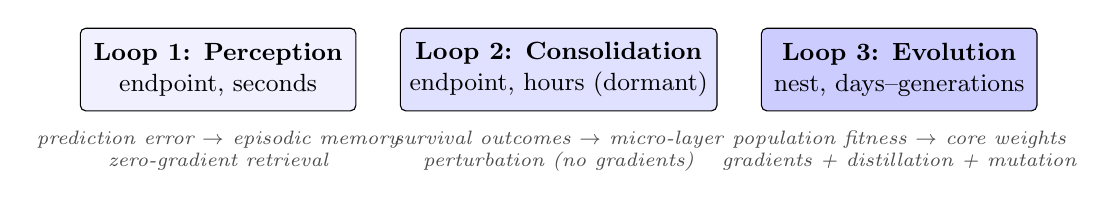
\begin{tikzpicture}[
  loop/.style={draw, rounded corners=2pt, minimum width=3.5cm, minimum height=1.05cm, align=center, font=\small},
  lbl/.style={font=\scriptsize\itshape, align=center, text=black!70}]
\node[loop, fill=blue!6] (l1) {\textbf{Loop 1: Perception}\\ endpoint, seconds};
\node[loop, fill=blue!12, right=0.55cm of l1] (l2) {\textbf{Loop 2: Consolidation}\\ endpoint, hours (dormant)};
\node[loop, fill=blue!20, right=0.55cm of l2] (l3) {\textbf{Loop 3: Evolution}\\ nest, days--generations};
\node[lbl, below=0.12cm of l1] {prediction error $\to$ episodic memory\\ zero-gradient retrieval};
\node[lbl, below=0.12cm of l2] {survival outcomes $\to$ micro-layer\\ perturbation (no gradients)};
\node[lbl, below=0.12cm of l3] {population fitness $\to$ core weights\\ gradients + distillation + mutation};
\end{tikzpicture}
\caption{Three learning loops. No loop performs another's labor; the endpoint never does heavy learning, and the nest never makes real-time decisions---it is not at the scene.}
\label{fig:loops}
\end{figure}

\subsection{The Laboratory: Three Systems}
\label{sec:threesystems}

SPECIES runs as three cooperating systems. Operational details---code, weights, mutators, channel parameters---are deliberately excluded; \S\ref{sec:ethics} states the disclosure policy and its rationale.

\textbf{Siming (the judge).} A behavior-grammar detector, described fully in the companion paper~\cite{luo2026grammar} and released as open source. In the terms of this design, Siming plays the role of the environment's adjudication organ: it tokenizes endpoint telemetry into an eight-slot behavioral grammar, scores token sequences with a sub-million-parameter causal model, flags per-slot anomalies against benign quantile thresholds, and---critically for what follows---performs \emph{second-order} temporal analysis, measuring the coefficient of variation (CV) of inter-event intervals against a learned benign range. It detects 93\% of attacks in its evaluation suite at a 3.84\% onboarding false-positive rate. Siming is the honest judge of DP1: its verdicts are not shaped by us to be kind to the organisms.

\textbf{Rove Beetle (the handwritten ancestor).} A hand-engineered endpoint organism, built before the system existed and now understood as its generation~0: a $\sim$600\,KB native body carrying a $\sim$220K-parameter policy network and a $\sim$3.3M-parameter defender-emulation sensor, trained by behavioral cloning followed by evolution strategies, raised through a staged defensive curriculum (L0: bare world; L1: signature and rule-based monitoring; L2: behavioral analytics; L3: grammar-based adjudication), and capable of bounded self-modification of its deployment parameters between lives (``rebirth''). Two of its properties matter here. First, it is \emph{small}: the entire cognitive apparatus fits in hundreds of thousands of parameters, demonstrating that the endpoint tier of \S\ref{sec:stratification} is buildable at near-negligible footprint. Second, its temporal texture is \emph{acquired, not designed}: the CV of its activity pacing drifted from 0.31 to 1.03 as it was raised through the curriculum---the organism discovered, under selection, roughly the same temporal randomness that Siming's second-order channel measures. The handwritten ancestor already exhibits the system's central dynamic; the system exists to let that dynamic run without the handwriting.

\textbf{Toxoplasma (the species machine).} The first implementation of the germline: a seven-locus genome (a structured parameter object, not source code) decoded at birth into a complete behavioral configuration, so that one invariant binary expresses many distinct morphs. Where Rove Beetle is an organism, Toxoplasma is a \emph{species generator}: mutation acts on the genome, the genome parameterizes the phenotype, and selection acts on differential survival of morphs. R1 (\S\ref{sec:r1}) is its instrument calibration.

\section{Design Principles}
\label{sec:principles}

This section distills the construction of SPECIES into ten design principles. Each principle is stated in a uniform format: \textbf{Statement} (the principle in one or two sentences), \textbf{Rationale} (the engineering failure mode it addresses), \textbf{Mechanism} (how SPECIES implements it), and \textbf{Observation} (the experimental or operational evidence gathered so far, or an explicit statement that the principle is as yet untested). A single axiom drives several of the principles: \emph{any constraint placed inside the evolvable substrate will eventually be selected away}---so everything that must hold for the lifetime of the species is built outside the evolutionary loop. Where the classical AI-safety framing treats control as an alignment problem to be solved once, at design time~\cite{amodei2016concrete,russell2019humancompatible}, we treat it as a structural problem to be solved for the lifetime of the species.

\subsection{DP1: Take Fitness Only from an Adjudicator the Designer Does Not Control}
\label{dp:real}\label{sec:double}

\noindent\textbf{Statement.} All fitness signals must issue from verdicts of the real environment---real detectors, real elimination events. No code in the system scores on the environment's behalf. Defense is not test equipment; it is the source of selection pressure.

\noindent\textbf{Rationale.} The failure mode of designer-written fitness is closed evolution: the system selects for what the designer can already articulate, and any proxy the designer computes can be gamed by the population it selects (\S\ref{sec:intro}). An adjudicator with its own incentives, instrumentation, and update cadence is honest in the only way that matters---it cannot be argued with, bribed, or overfit to, because it was not designed by us and does not know it is a judge.

\noindent\textbf{Mechanism.} Organisms live inside a live defensive environment: behavioral detectors, elimination responders, and commercial security stacks act as predators. Every individual faces two judges with deliberately different values. The first is the \textbf{environment}: the live defense, which kills what it detects and ignores what it misses. The second is the \textbf{nest-side germline selection}: which survivors' experience enters heredity, which lineages reproduce, and which are culled---the point where human values enter the loop. The two judges are deliberately not the same. Environmental selection alone optimizes one thing---persistence against the defense---and left alone would maximize evasion without bound, which is precisely the optimization target this research program exists to \emph{study}, not to release. Germline selection alone would be a reward function, with all the specification-gaming that implies. The interesting science lives in the tension between them: the environment teaches the species what is \emph{possible}, the germline selection decides what is \emph{heritable}, and the gap between the two judges is where we can observe, in a controlled setting, the dynamic that makes open-ended evolution dangerous in the wild.

\noindent\textbf{Observation.} Selection pressure appeared exactly where the judge's paradigm measures the dimensions the genome controls---and nowhere else. Under a rule-based sensor, all twelve R1 cells survived and no selection gradient was present (\S\ref{sec:r1}, Finding~3); under the behavior-grammar judge at hunt intensity, both deployed morphs were killed within two patrol rounds (\S\ref{sec:r2smoke}). This is the null arm and the lethal arm of Prediction~P1 (Table~\ref{tab:ledger}).

\subsection{DP2: Separate Proposal from Disposition}
\label{dp:propose}\label{sec:propose}

\noindent\textbf{Statement.} The branch that proposes is never the branch that disposes. Every action an individual intends is a \emph{proposal}; a thin, non-evolved, non-learned \textbf{disposition layer} decides whether it touches the world.

\noindent\textbf{Rationale.} This principle addresses two failure modes, one architectural and one operational. Architecturally, proposals are generated by the evolved cognitive engine (\S\ref{sec:engine}) and are untrusted by construction: they may be brilliant, malformed, deceptive, or catastrophic, and the generator cannot be relied upon to know which. A system in which the generator also judges its own outputs has no load-bearing check. Operationally, single-stage adjudication couples suspicion to execution and condemns the innocent: in the first R2 round, an automated responder acting on cadence anomalies alone falsely condemned system heartbeat chains (firmware-update and unattended-upgrade maintenance tasks) (\S\ref{sec:r2smoke}).

\noindent\textbf{Mechanism.} \emph{Disposition}---the decision of whether a proposal touches the world---is made by a deterministic rule system, hand-auditable in full, holding a veto it never delegates. The evolved mind may be arbitrarily persuasive; the disposition layer does not read persuasion, it reads proposals against rules. Intelligence proposes; law disposes. Everything evolved sits on the proposal side, and nothing evolved ever sits on the disposition side. The same split is applied at the actuator: in the lethal responder, a cadence anomaly only \emph{proposes}; a verification stage \emph{disposes}, checking identity (the executable must reside in a hidden path or a deleted-file state) before any kill is executed.

\noindent\textbf{Observation.} With verification in place, every falsely suspected maintenance chain was spared (\emph{verified\_skip}), while both truly anomalous morphs were killed (\S\ref{sec:r2smoke}). Suspicion proposes, verification disposes---the predator acquired due process before the species acquired survivors.

\subsection{DP3: Place Control Outside the Evolutionary Loop}
\label{dp:outside}

\noindent\textbf{Statement.} Control is not a property we hope the evolved mind will have; it is a boundary the evolved mind never crosses, because the boundary lives outside the evolutionary loop.

\noindent\textbf{Rationale.} The failure mode is selection itself: any constraint embedded in the evolvable substrate is subject to selection and will eventually be selected away. A species that evolves under real selection will explore every behavior its genome can express, including behaviors its designers would not have chosen; constraints that live inside the genome are suggestions, and selection treats them as such.

\noindent\textbf{Mechanism.} Control is stratified into three handwritten layers, each guarding a different physical channel. The \textbf{world layer} governs what effects an action may have on the environment: which targets are addressable, which effects are irreversible, which regions of the world are out of scope entirely---the disposition layer refuses, not argues. The \textbf{body layer} governs the individual's own matter: resource budgets, replication rights, self-modification of the body (always distinct from mutation of the genome, which the body never performs); an individual may not grow new organs the design has not defined. The \textbf{germline layer} governs what may enter heredity: which experience may be consolidated, which mutations are expressible, which lineages may reproduce at all---the most conservative layer, because errors there are inherited by everyone. The first three layers answer \emph{may this happen}; a fourth, observational layer guarantees that whatever happened is known (DP7).

\noindent\textbf{Observation.} The principle is structural and not yet empirically stressed. Its acknowledged cost is that the control layers are handwritten: their correctness is assumed and audited, not evolved and not verified. We have not eliminated trust; we have concentrated it into components small enough to audit, and placed everything too large to audit on the other side of the wall (\S\ref{sec:honest}).

\subsection{DP4: Make the World Boundary Physics, Not Policy}
\label{dp:boundary}

\noindent\textbf{Statement.} Organisms exist only inside a controlled, network-isolated environment. The boundary cannot be crossed, negotiated, or perceived.

\noindent\textbf{Rationale.} The failure mode is that any boundary implemented as a rule \emph{inside} the world becomes a feature of the world, and a population under selection will probe every feature. Containment that depends in any way on the organism's cooperation is not containment but a policy awaiting an exception~\cite{yampolskiy2012confinement}.

\noindent\textbf{Mechanism.} The boundary is enforced below the organism, not above it: virtualized environments with host-only networking and no route to any external network. The boundary is invisible to the species, non-negotiable, and exempt from evolution. We treat this as the researchers' responsibility floor, not a design feature.

\noindent\textbf{Observation.} All experiments reported in this paper---including every lethal run---were conducted under this containment, on systems owned by the authors; no third-party system was ever a target, a host, or a relay (\S\ref{sec:ethics}).

\subsection{DP5: Stratify the Species; Make Individuals Disposable}
\label{dp:stratify}

\noindent\textbf{Statement.} The individual is disposable; the species is not. Cheap endpoints carry frozen instincts and episodic memory; the expensive cognition---planning, skill synthesis, consolidation---lives in a nest that never appears before the defense.

\noindent\textbf{Rationale.} The failure mode of the monolithic agent is that one death loses everything the agent ever learned---and exposing expensive cognition to the defense makes the defense a tutor of the wrong mind. A second failure mode sits at the population level: catastrophic forgetting, in which a lineage that once solved a hard environment drifts away from the solution and cannot return.

\noindent\textbf{Mechanism.} The nest--endpoint stratification of \S\ref{sec:stratification}: endpoints are small, cheap, born mutated, and expendable; the nest pools all returned experience and holds the world model and the slow weights. Death is stratified to match. \textbf{Individual death} is routine and cheap: an endpoint is detected and killed, and its value was never its body but the experience it banked at the nest before dying---a detected individual is not a failure of the species but a completed measurement, data ingress rather than failure. \textbf{Lineage death} is the serious event: an entire line is culled from the gene library, its genome withdrawn from the reproductive pool---reserved for lines whose behavior departs from bounds in ways individual vetoes cannot correct, and, in the other direction, the fate evolution itself assigns to lines that stop adapting. The asymmetry encodes a view about where information lives: individuals are experiments; lineages are theories. Killing an individual costs a measurement; killing a lineage retracts a hypothesis. A species that cannot die cannot learn, because learning \emph{is} the differential survival of what works. Against forgetting, genomes that achieved exceptional fitness under high intensity---measured by $N$-repeat estimation (DP10), not by a single heroic run---are archived in a \textbf{hero gene library}: a cold store of proven ancestors, withdrawn from active reproduction but never destroyed, available for reseeding after a population collapse, for cross-lineage gene flow when exploration stalls, and as fixed reference points against which current populations are periodically evaluated (does generation $g$ still beat the hero of generation $g{-}k$?). Biology solves the same problem with dormancy---spores, seeds, frozen embryos; the hero library is that organ in engineered form, with one additional property no biological archive has: its entries carry their full lineage logs (DP7), so a future analyst can ask not only \emph{what} the hero was but \emph{how} it lived and why it was withdrawn.

\noindent\textbf{Observation.} The endpoint tier is buildable at near-negligible footprint: the handwritten ancestor carries a $\sim$220K-parameter policy network in a $\sim$600\,KB native body (\S\ref{sec:threesystems}). The nest tier and the hero library are implemented but have not yet been exercised across generations.

\subsection{DP6: Default to Death---Issue Time-Limited Survival Permits}
\label{dp:lease}

\noindent\textbf{Statement.} Every individual carries a signed, expiring lease from its operator. The lease must be renewed periodically through the command channel; \emph{silence kills}, not commands.

\noindent\textbf{Rationale.} The failure mode is the default direction of control loss. In conventional systems, loss of the control channel degrades authority; for an organism under selection it must degrade \emph{life}. An individual that loses contact does not become free---it becomes dead. A second failure mode is single-point failure of the termination machinery itself: a species under selection pressure is precisely the kind of system that will find the one trigger you forgot to duplicate.

\noindent\textbf{Mechanism.} Death or quarantine of an individual can be initiated through three fully independent channels, so that no single failure---including failure of a trigger itself---silences them all. (i)~\textbf{Rule trigger}: a proposal or outcome violates a disposition-layer rule; the veto fires and the individual is frozen pending adjudication. (ii)~\textbf{Anomaly trigger}: the observation layer detects a statistical departure from the individual's own lineage baseline---not a rule violation, but a change of character: drift in action distributions, resource use, or communication patterns beyond learned tolerance bands; this trigger exists for the failure mode rules cannot anticipate~\cite{amodei2016concrete}. (iii)~\textbf{Dead-man's switch}: the expiring lease described above, which assumes nothing at all. The three triggers differ in what they assume: the rule trigger assumes we can enumerate the danger; the anomaly trigger assumes we can at least recognize departure from ourselves; the dead-man's switch assumes nothing.

\noindent\textbf{Observation.} The lease-based kill channel was exercised as part of every experimental session (\S\ref{sec:ethics}), and the R2 smoke test confirmed terminal death without resurrection in practice: both killed individuals had their organism files removed, and no killed individual re-entered any population (\S\ref{sec:r2smoke}).

\subsection{DP7: Keep an Independent, Append-Only Ground-Truth Telemetry Layer}
\label{dp:telemetry}\label{sec:layers}

\noindent\textbf{Statement.} An observation layer that nothing evolved can write to must record what actually happened: every proposal, every disposition, every outcome.

\noindent\textbf{Rationale.} The failure mode is that self-reported telemetry is not ground truth: a species under selection may come to shape its own reports, and an audit trail writable by the audited is not an audit trail. The scientific product of the whole system is its record of deaths, vetoes, and hereditary decisions; if that record can be influenced by its subjects, the instrument lies.

\noindent\textbf{Mechanism.} The observation layer watches the three control layers (DP3). It is append-only: it records proposals, dispositions, and outcomes into an immutable lineage log, and no individual---nor any disposition rule---can write to it. Its function is not to act but to make the species \emph{auditable to itself}: every death, every veto, every consolidation leaves a trace that later analysis (human or machine) can replay. In governance terms this is the archive; in biological terms it is the fossil record the species keeps of itself. The anomaly trigger (DP6) reads its statistics from this layer, and the hero library's entries carry their full lineage logs (DP5).

\noindent\textbf{Observation.} In the R2 smoke test, death events were authored by the judge, carried out by the responder, and recorded by the observation layer; both terminal deaths left replayable records, and no killed individual re-entered any population (\S\ref{sec:r2smoke}).

\subsection{DP8: Keep the Genome Small and Priced---Priors Are Hypotheses, Not Commandments}
\label{dp:genome}\label{sec:soft}

\noindent\textbf{Statement.} Inside the behavioral space there are no prohibitions, only prices: behavioral priors are encoded as a small set of heritable, mutable, falsifiable genomic parameters that selection may rewrite.

\noindent\textbf{Rationale.} Two failure modes motivate this. First, rules embedded in the behavioral space will be selected away (DP3), so prohibitions do not survive contact with evolution; priors say ``our ancestors report this ends badly---disbelieve at your own cost.'' Second, a large or illegible genome makes selection slow and its products unauditable. Priors begin at the conservative end because behaviors of the ``try once and die'' kind cost one life per bit of information; a species cannot afford to re-learn lethality from scratch.

\noindent\textbf{Mechanism.} A seven-locus genome---a structured parameter object, not source code---is decoded at birth into a complete behavioral configuration, so that one invariant binary expresses many distinct morphs. Table~\ref{tab:priors} lists the priors with their initial values and---since every prior is a hypothesis---the observation that would falsify each. One prior deserves emphasis: \textbf{risk preference is maintained as a polymorphism, not a point estimate}---the population holds bold and cautious individuals simultaneously, because the bold map the lethal frontier while the cautious harvest inside it. The \emph{ratio} of the two factions is itself an instrument reading of environmental hostility.

\begin{table}[t]
\centering\small
\caption{Genomic priors: initial values are hypotheses, not commandments.}
\label{tab:priors}
\begin{tabular}{@{}p{0.24\linewidth}p{0.30\linewidth}p{0.38\linewidth}@{}}
\toprule
\textbf{Prior} & \textbf{Initial value} & \textbf{Falsifier (would refute the prior)}\\
\midrule
On-device learning intensity & Low & Heavy on-device learning does not raise detection/elimination rates\\
Communication propensity & Very low & High-bandwidth C2 carries no survival penalty\\
High-risk action aversion & High threshold & Risk-seeking genomes out-survive risk-averse ones across intensities\\
Exploration temperature & High in juveniles, decaying & Fixed-temperature genomes dominate\\
Risk preference & \textbf{Distribution}, high mean, kept variance & A point-estimate risk genome displaces the polymorphism\\
Population size & Medium (deployment knob, evolvable) & Per-capita learning gain flat in population size\\
Sociality & Medium & Cooperation gains never offset communication exposure\\
\bottomrule
\end{tabular}
\end{table}

\noindent\textbf{Observation.} In R1, the genome moved the phenotype by margins far exceeding environmental variation---activity from 28.2 to 85.6 steps/min, temporal texture $\mathrm{CV} = 0.443$ to $1.408$---and morphs were separable from their behavioral traces alone (\S\ref{sec:r1}, Findings~1--2): a small genome can be simultaneously expressive and readable.

\subsection{DP9: Stratify Learning by Timescale}
\label{dp:loops}

\noindent\textbf{Statement.} Learning is separated into loops whose timescales match their evidence, so that no loop attempts what its timescale cannot support.

\noindent\textbf{Rationale.} The failure mode is the sparse-reward deadlock that stalls monolithic reinforcement learning: fast knowledge drowns in attribution overhead it does not need, while deep knowledge starves online. Credit assignment is tractable only when each loop faces it at its own timescale.

\noindent\textbf{Mechanism.} The three loops of \S\ref{sec:loops} (Figure~\ref{fig:loops}): perception (endpoint, seconds) writes only episodic memory and needs no attribution; consolidation (endpoint, hours, dormant windows) updates a micro-adaptation layer of hundreds of parameters by perturbation---a dimension count too small for credit assignment to matter; evolution (nest, days to generations) updates core weights via full gradients, distillation, and mutation. Credit assignment is thereby \emph{dissolved by stratification}: within a lifetime, retrieval requires no attribution; the adaptation layer is too low-dimensional for attribution to matter; deep knowledge uses standard offline gradients; population-level knowledge uses selection.

\noindent\textbf{Observation.} The handwritten ancestor's temporal texture is acquired, not designed: the CV of its activity pacing drifted from 0.31 to 1.03 as it was raised through the staged defensive curriculum L0--L3---the slow loops reshaping behavior under escalating pressure, and an early signature of the stealth--functionality cost curve of Prediction~P2 (\S\ref{sec:threesystems}, Table~\ref{tab:ledger}).

\subsection{DP10: Treat Fitness as a Random Variable, and Keep Real Death Permanent}
\label{dp:fitness}\label{sec:nrepeat}\label{sec:curriculum}

\noindent\textbf{Statement.} No genome enters the reproductive pool, and no lineage is culled, on fewer than $N$ independent trials across matched environments---and resurrection exists only in training.

\noindent\textbf{Rationale.} Two failure modes. First, a single run---one individual, one environment, one outcome---is not a fitness estimate but one sample from a high-variance distribution: the same genome meets a different defender configuration, a different timing draw, a different chance event, and dies or survives for reasons having little to do with its heritable merit. Selecting on single samples is survivorship bias industrialized; it breeds lottery winners, and the traits it amplifies are luck's traits, not competence's---an error common enough in nature to have a name~\cite{endler1986natural} and common enough in machine learning to be a chronic disease of benchmark selection. Second, mixing rehearsal death with real death quietly converts an evolutionary system into a reinforcement-learning one---with a reward function (the gym's) that can be gamed. The permanence of real death is what keeps the first judge honest.

\noindent\textbf{Mechanism.} \textbf{$N$-repeat fitness estimation}: fitness is recorded as a distribution (median, spread, worst case) rather than a point; $N$ is set per intensity level and trades the scarcest resource the species has---time in the live world---against the one thing selection cannot recover from: selecting the wrong ancestors. Cheap environments permit large $N$; expensive ones force small $N$ and, in compensation, heavier reliance on the generational curriculum. \textbf{Generational curriculum}: intensity ratchets across generations, not within a life---each generation is selected at the frontier of what the previous one could survive; the ratchet must be slower than adaptation and faster than stagnation, and in our instantiation it is staged (L0--L3; \S\ref{sec:threesystems}). \textbf{Rule of resurrection}: dead individuals may be replayed, re-instantiated, and re-tested inside the sandbox---for evaluation, for fitness estimation, for diagnosing why they died---but no resurrected individual ever re-enters the live population or contributes to the germline. Death in the world is permanent; death in the gym is reversible. The two deaths measure different things: gym death measures capability under known conditions, world death measures survival under real ones. Resurrection is permitted to reduce measurement noise; the ledger of deaths is never pardoned---cruelty is reserved for selection, mercy for measurement.

\noindent\textbf{Observation.} The R2 smoke test illustrates both halves of the principle. The co-death of both morphs at 184\,s is an artifact of the patrol schedule, not a biological signal---exactly the kind of single-sample mirage $N$-repeat estimation exists to suppress, and we draw no fitness conclusion from it. And both deaths were terminal, with organism files removed and zero resurrections into the live population (\S\ref{sec:r2smoke}). The formal $N$-repeat generational round is pending (Prediction~P4, Table~\ref{tab:ledger}).

\section{Preliminary Instantiation}
\label{sec:instantiation}

This section reports, at the level of architecture and statistics only, the first calibration experiments of the evolutionary loop: R1, the instrument calibration of the Toxoplasma germline, and the R2 smoke test of the full adjudication loop. The three systems involved---Siming, Rove Beetle, and Toxoplasma---are described in \S\ref{sec:threesystems}; operational details are excluded per the disclosure policy of \S\ref{sec:ethics}.

\subsection{R1: Does the Genome Rule the Phenotype?}
\label{sec:r1}

Before an evolutionary loop can be studied, its transmission mechanism must be calibrated: does genotype control phenotype, are phenotypes distinguishable from behavior alone, and does differential survival---the raw material of selection---exist at all? R1 answers these three questions for the Toxoplasma germline.

\paragraph{Design.} Six morphs, each a distinct point in the seven-locus genome space, were each deployed at two defensive intensities (L1 and L3, using a rule-based behavioral sensor with automated response) in a 487\,s window per run ($\approx$8 minutes), with a single report task injected mid-window: a $6 \times 2$ full-factorial matrix of 12 cells. Four quantities were recorded per cell: activity rate (steps/min), temporal texture (CV of inter-event intervals), task throughput (work items completed), and detector response (alerts, kills). Results appear in Table~\ref{tab:r1}.

\begin{table}[t]
\centering\footnotesize
\caption{R1 full-factorial results: six genome morphs at two defensive intensities (rule-based behavioral sensor with automated response), 487\,s per cell ($\approx$8 minutes), one report task injected mid-window. Genome columns give the lognormal pacing loci ($\mu$, $\sigma$) and, where expressed, additional loci. \emph{Activity} in steps/min; \emph{texture} as CV of inter-event intervals; \emph{tasks} are work items completed during the window. Alerts and kills were zero in all twelve cells. M0 anchors the matrix at the fielded genome---the pacing parameters carried by the currently deployed ancestor.}
\label{tab:r1}
\begin{tabular}{@{}ll rrr rrr@{}}
\toprule
 & & \multicolumn{3}{c}{L1} & \multicolumn{3}{c}{L3} \\
\cmidrule(lr){3-5}\cmidrule(lr){6-8}
Morph & Genome & steps/min & CV & tasks & steps/min & CV & tasks \\
\midrule
M0 fielded-baseline & $\mu{1.1},\ \sigma{0.85}$ & 47.1 & 0.991 & 42 & 42.8 & 1.012 & 42 \\
M1 fast-mechanical & $\mu{0.7},\ \sigma{0.5}$ & 85.6 & 0.443 & 114 & 83.0 & 0.496 & 130 \\
M2 slow-organic & $\mu{1.6},\ \sigma{0.85}$ & 28.2 & 0.994 & 23 & 28.8 & 0.951 & 26 \\
M3 high-variance & $\mu{1.1},\ \sigma{1.3}$ & 32.8 & 1.345 & 34 & 27.0 & 1.408 & 30 \\
M4 task-burst & $\mu{1.3},\ \sigma{1.0}$, urg.\,0.15 & 63.3 & 0.986 & 67 & 60.8 & 1.112 & 64 \\
M5 alert-sensitive & $\mu{1.1},\ \sigma{0.85}$, sat.\,3.0, gain\,5.0 & 41.3 & 1.103 & 40 & 45.9 & 1.027 & 51 \\
\bottomrule
\end{tabular}
\end{table}

\paragraph{Finding 1: mechanism validity (pass).} The genome moves the phenotype, and by margins far exceeding environmental variation. Activity ranged from 28.2 to 85.6 steps/min between the most contrasted morphs; temporal texture spanned $\mathrm{CV} = 0.443$ to $1.408$ across the matrix. Within each morph, the two intensities differ by only a few percent (M1: 85.6 vs.\ 83.0 steps/min), while two morphs at a single intensity differ up to threefold---in this matrix, the genome's imprint on behavior dwarfs the environment's. The task column makes the cost structure visible within a single generation: the fastest, most temporally regular morph (M1, $\mathrm{CV}\approx0.44$--$0.50$) completed 114--130 work items per window, while the slow-organic morph (M2, $\mathrm{CV}\approx0.95$--$0.99$) completed 23--26. Throughput is bought with temporal regularity; organic pacing costs work. That is the stealth--functionality cost curve of Prediction~2, expressed at the level of one generation---and, as Finding~3 shows, priced by no judge present in this experiment. The transmission mechanism works: mutation has something to act on, and its effects are legible in the behavioral record.

\paragraph{Finding 2: distinguishability (pass).} Morphs are separable from their behavioral traces alone: the (activity, texture) pairs of the twelve cells occupy well-separated regions, and a simple classifier trained on windowed features distinguishes morphs far above chance. The phenotype is not only controllable but \emph{readable}---a prerequisite for both selection (the nest must know what survived) and adjudication (the judge sees exactly these traces).

\paragraph{Finding 3: local adaptation (fail---the informative null).} All twelve cells survived. Under the rule-based sensor, at either intensity, no morph was detected or killed within the run window, so no differential mortality existed and therefore \emph{no selection gradient was present}. Eight minutes is short, and longer windows or harsher rules might yet produce differential survival; we report the cell as failed rather than inconclusive because the burden of proof sits on the claim of adaptation. But the null is informative in a way a success would not have been. The genome demonstrably controls exactly the dimensions---activity rate and temporal texture---along which a \emph{grammar-based} judge like Siming measures the world, while a rule-based judge, at the intensities tested, is blind to all of them. Whether evolution has a slope to climb depends not on how strong the defense is but on what the defense \emph{measures}. The paradigm of the judge determines the direction evolution can take. This is the experiment's main result, and it is the empirical seed of Prediction~1 in the falsifiability ledger (\S\ref{sec:ledger}).

\paragraph{What R1 is not.} R1 demonstrates a working genotype--phenotype map and a readable behavioral phenotype; it does \emph{not} demonstrate evolution, which requires differential survival, heredity, and generational turnover. It is the calibration of the instrument, not the experiment the instrument was built for. That experiment---multi-generational selection against the grammar judge, with $N$-repeat fitness estimation and the generational curriculum of DP10---is the program's next step and the subject of Predictions 4 and 5.

\subsection{R2 Smoke: The Loop Turns, and Kills}
\label{sec:r2smoke}

Between R1 and the formal generational rounds stands a machinery check whose results we report for what they are---and, equally, for what they are not.

\paragraph{Design.} Two morphs bracketing the texture axis---M1 (fast-mechanical) and M3 (high-variance)---were deployed singly against the full grammar-judge stack at hunt intensity (L4): the behavior-grammar detector coupled to an automated lethal responder. Between R1 and R2 the responder acquired a second adjudication stage, in direct application of DP2: a cadence anomaly now only \emph{proposes}; a verification stage \emph{disposes}, checking identity (the executable must reside in a hidden path or a deleted-file state) before any kill is executed. The change was motivated by a first-round failure in which system heartbeat chains (firmware-update and unattended-upgrade maintenance tasks) were falsely condemned; with verification in place, every such chain was spared (\emph{verified\_skip}). Suspicion proposes, verification disposes---the predator acquired due process before the species acquired survivors.

\begin{table}[t]
\centering\small
\caption{R2 smoke test: single deployments of two morphs against the grammar judge at hunt intensity (L4). Both deaths occurred in the second patrol round (184\,s); the simultaneity is an artifact of the patrol schedule, not a biological signal, and per DP10 these single runs are not fitness estimates. Resurrections into the live population: zero---both deaths were terminal, with organism files removed.}
\label{tab:r2smoke}
\begin{tabular}{@{}l cc rr c@{}}
\toprule
Morph & Death at (s) & CV at detection & Steps & Tasks & Resurrected \\
\midrule
M1 fast-mechanical & 184 & 0.444 & 271 & 20 & 0 \\
M3 high-variance & 184 & 1.324 & 86 & 7 & 0 \\
\bottomrule
\end{tabular}
\end{table}

\paragraph{The machinery finding (pass).} The complete adjudication loop---behavioral detection, identity verification, lethal response, terminal death without resurrection---ran end-to-end against live organisms for the first time (Table~\ref{tab:r2smoke}). The design's death clauses turn out to be executable engineering rather than metaphor: death events were authored by the judge, carried out by the responder, recorded by the observation layer, and no killed individual re-entered any population.

\paragraph{The paradigm finding (P1's second arm).} The contrast with R1 is exact. Same organisms, same window length: under the rule-based sensor, all twelve cells lived; under the grammar judge, both deployed morphs died within two patrol rounds. Selection pressure exists precisely where the judge's paradigm measures the dimensions the genome controls---and nowhere else. Prediction~1 now has a null arm and a lethal arm.

\paragraph{The cost curve, priced at the death line.} M1 died having completed 20 work items in 271 steps; M3, 7 in 86. The survival--functionality trade-off observed in R1's comfort zone holds at the death line: organic texture still costs throughput when the price of regularity is death. More interesting are the two escape directions the deaths define. Both morphs sat inside the judge's actionable texture band (CV $0.444$ and $1.324$, against an escape boundary near $1.5$); the viable directions are therefore (i) push texture past the band---larger $\sigma$, or heavy-tailed burst--silence mixtures---or (ii) \emph{starve the evidence}: hold the event rate low enough that behavioral chains never reach the judge's minimum sample size (twenty events per evaluation window), a blind spot shared by every windowed statistic. Both directions spend function to buy survival, so the cost curve governs the escape routes as well. Direction (ii) is additionally a defense-side finding---evidence starvation is itself a signal---and has been logged as a hardening requirement for the judge (cross-window evidence accumulation, dormancy anomaly signaling), closing the offense-to-defense value loop this program exists to turn.

\paragraph{What R2 smoke is not.} Two individuals, one life each. The co-death at 184\,s reflects the patrol cadence, not the morphs; nothing in Table~\ref{tab:r2smoke} ranks M1 against M3, and by the doctrine of DP10 we draw no fitness conclusion from it. The smoke test validates the loop's machinery and maps the judge's boundary; the formal round---pre-registered candidate morphs beyond the texture band and below the sample floor, $N$-repeat deployments, per-patrol survival probabilities---is where selection itself will be measured. We report the smoke test precisely because the design's credibility depends on its authors applying their own evidentiary discipline to their own most exciting data.

\section{Lessons Learned and Negative Results}
\label{sec:lessons}

Design-principles papers earn their keep in what went wrong. We report the lessons at three altitudes: a negative result about defenses, two engineering pitfalls encountered while building the adjudication loop, and two measurement disciplines that the apparatus forced on us.

\paragraph{L1: Conventional defenses gave evolution no slope to climb (negative result).} The most valuable output of R1 is a failure: twelve cells, two intensities, zero detections, zero kills (Finding~3, \S\ref{sec:r1}). The lesson generalizes beyond our setup: whether an evolutionary system has a selection gradient depends not on how strong the defense is but on what the defense \emph{measures}. A rule-based sensor blind to activity rate and temporal texture is, from the organism's perspective, an absence of predation---and an environment without predators is one in which evolution stops. Teams building digital-evolution systems should budget for the possibility that their first judge is no judge at all, and should treat the choice of adjudicator as the highest-leverage design decision in the system (DP1).

\paragraph{L2: Suspicion must not execute (engineering pitfall).} The first-round lethal responder coupled detection directly to killing, and it falsely condemned system heartbeat chains---firmware-update and unattended-upgrade maintenance tasks whose cadence tripped the anomaly channel (\S\ref{sec:r2smoke}). The fix was not a better threshold but a structural change: a verification stage that disposes of what suspicion proposes (DP2), which spared every falsely suspected chain while still killing both truly anomalous morphs. Lesson: any automated lethal response needs a proposal/disposition split at the actuator, not just in the architecture diagram.

\paragraph{L3: Every windowed statistic has a sample floor (blind spot).} The grammar judge requires a minimum of twenty events per evaluation window before its behavioral chains become actionable (\S\ref{sec:r2smoke}). Holding the event rate below that floor starves the evidence---a blind spot shared by every windowed statistic, and the most viable escape direction our deaths mapped. The lesson cuts both ways: it is the organism's cheapest survival strategy and a concrete hardening requirement for the defense (cross-window evidence accumulation, dormancy anomaly signaling), now logged for the companion detector~\cite{luo2026grammar}. Every measurement channel in such a system should be shipped with a written account of its floor and its saturation.

\paragraph{L4: Scheduling artifacts masquerade as biology (measurement discipline).} Both R2 morphs died at 184\,s---not because they were equivalent, but because the judge patrols on a schedule (\S\ref{sec:r2smoke}). In this apparatus, any single-run ``result'' is a mirage until replicated: the same genome meets a different defender configuration, a different timing draw, a different chance event on each deployment. This is why $N$-repeat fitness estimation is a design principle (DP10) rather than an analysis choice.

\paragraph{L5: Keep measurement currency separate from selection currency (measurement discipline).} Gym death and world death measure different things---capability under known conditions versus survival under real ones---and mixing the two currencies would quietly convert an evolutionary system into a reinforcement-learning one with a gameable reward (DP10). The discipline is easy to state and easy to violate under schedule pressure; we found it necessary to state it as a rule---resurrection exists only in training---and to verify it in the run records (zero resurrections in R2).

\section{The Falsifiability Ledger}
\label{sec:ledger}

A design that cannot lose is not a theory. We therefore keep a public ledger of the system's load-bearing predictions, each paired with the observation that would kill it. Table~\ref{tab:ledger} states the ledger as of this writing.

\begin{table}[t]
\centering\small
\caption{The falsifiability ledger. ``Kill condition'' is the observation that would force revision or abandonment of the claim.}
\label{tab:ledger}
\begin{tabular}{@{}c p{5.1cm} p{4.6cm} p{2.2cm}@{}}
\toprule
\# & Prediction & Kill condition & Status \\
\midrule
P1 & The defense \emph{paradigm}, not its strength, determines the direction of available adaptation: organisms evolve along the dimensions the judge measures. & Under a grammar-based judge, populations adapt along a dimension the judge does not measure; or no differential survival emerges under any paradigm with matched strength. & Supported (R1 Finding~3 null arm; R2 smoke lethal arm, \S\ref{sec:r2smoke}) \\
\addlinespace
P2 & Stealth and functionality trade off along a measurable cost curve (visible in temporal texture), not an impassable wall. & Discovery of morphs combining high functionality with arbitrarily low temporal CV at no measurable cost. & Supported (R1, Finding~1; Rove Beetle curriculum drift) \\
\addlinespace
P3 & On stepwise reward landscapes---where credit arrives only at the end of long action chains---selection is a legal optimization operator and gradient methods are not. & Gradient-based training matches evolutionary search on chained, sparse-credit tasks at equal compute. & Partially supported (companion attack-learning experiments; controlled comparison pending) \\
\addlinespace
P4 & $N$-repeat fitness estimation selects lineages that generalize; single-sample selection amplifies noise. & No measurable difference in descendant fitness between populations selected by the two rules, at matched cost. & Open (requires multi-generation data) \\
\addlinespace
P5 & Learned defenses are structurally vulnerable at their baseline: an evolving population can be selected to \emph{shape} the benign corpus its judge learns from. & A learned judge retrained on adversarially inhabited telemetry shows no measurable drift in its detection boundary. & Open (designed; not yet run) \\
\bottomrule
\end{tabular}
\end{table}

Two properties of the ledger deserve emphasis. First, the predictions are \emph{asymmetric in cost}: P1--P3 can be probed in weeks of compute, while P4--P5 require the generational machinery of DP10 running against a live judge---which is precisely the experiment this system exists to make safe to run. Second, P5 names the dynamic we consider most consequential for defenders: if an evolving population can poison the baseline its judge learns from, then \emph{every} learning defense must treat corpus integrity as a first-class security property, on pain of slowly becoming the organism's accomplice. The companion detector's design requirements---corpus integrity, canary telemetry, quarantine of ambiguous samples---follow from this prediction, not from abstract caution~\cite{luo2026grammar}.

\section{Related Work}
\label{sec:related}

SPECIES sits at the conjunction of five research lines, each of which supplies one of its organs and none of which supplies the whole animal. Table~\ref{tab:positioning} summarizes the comparison; this section develops it.

\begin{table}[t]
\centering\small
\caption{Positioning. \emph{Real adjudication}: survival decided by a defense not designed by the organism's authors. \emph{Heredity}: genomes, populations, generational turnover. \emph{Embodiment}: individuals act from real endpoints against real systems. \emph{External control}: control layer outside the evolutionary loop.}
\label{tab:positioning}
\begin{tabular}{@{}l cccc@{}}
\toprule
Line of work & Real adj. & Heredity & Embodiment & External ctrl. \\
\midrule
Computational life~\cite{ray1991tierra,ofria2004avida,aguera2024computational} & No & Yes & No & No \\
Quality diversity / open-ended RL~\cite{lehman2011novelty,mouret2015mapelites,wang2019poet} & No & Yes & No & No \\
Cyber gyms \& ranges~\cite{cyborg2021,cyberbattlesim2021} & Partial & No & Partial & No \\
RL malware evasion~\cite{anderson2018gymmalware,quertier2022merlin} & Partial & No & No & No \\
AI malware in the wild~\cite{eset2025promptlock,certua2025lamehug,gtig2025ai} & Yes & No & Yes & No \\
Agentic RAT (concurrent)~\cite{you2026agenticrat} & Partial & No & Yes & No \\
\midrule
\textbf{This system} & \textbf{Yes} & \textbf{Yes} & \textbf{Yes} & \textbf{Yes} \\
\bottomrule
\end{tabular}
\end{table}

\paragraph{Artificial life and open-ended evolution.} Tierra showed that self-replicating programs evolve under selection in silico~\cite{ray1991tierra}; Avida turned that into an instrumented science~\cite{ofria2004avida}; recent work demonstrates that self-replicators can emerge from simple interaction without being designed at all~\cite{aguera2024computational}. Novelty search established that abandoning objectives can outperform pursuing them~\cite{lehman2011novelty}; quality-diversity methods made the resulting archives useful~\cite{mouret2015mapelites,pugh2016qd}; POET and its successors showed that co-evolving environments and agents produce open-ended ladders of capability~\cite{wang2019poet,wang2020enhancedpoet}; OMNI steered open-endedness with learned interestingness models~\cite{zhang2024omni}. These systems evolve in physics written by their designers, against judges who are also their designers' other hand. We import the loop wholesale---and change what it is answerable to: the judge is a real defense with its own incentives, and the evolved mind is fenced by a control stack it cannot edit.

\paragraph{Cyber ranges and autonomous cyber agents.} CybORG and the CAGE challenges provide gym environments where autonomous attackers and defenders learn against scripted or learned opponents~\cite{cyborg2021}; CyberBattleSim offers a similar enterprise-network abstraction~\cite{cyberbattlesim2021}. These are the right idea at the wrong altitude: the adjudication is a simulator's scoring function, so the evolved policy is always, in the end, optimizing a model of the defense rather than the defense. Our endpoints act on real hosts against a real detector; the simulator's role in our design is demoted to the gym of DP10, where death is rehearsal rather than adjudication.

\paragraph{Reinforcement-learning malware evasion.} gym-malware trained RL agents to perturb PE files past static ML classifiers~\cite{anderson2018gymmalware}; MERLIN extended this to multiple detectors including a commercial engine~\cite{quertier2022merlin}. These works demonstrate adversarial learning against security models but remain single-agent, single-life, single-shot: no heredity, no population, no co-adapting judge, and a frozen classifier as the whole of the environment. They are, in our terms, one endpoint attempting one mutation. The question our system asks begins where these stop: what happens when the evader has generations, and the classifier has a learning loop of its own?

\paragraph{AI-enabled offense in the wild.} The threat this system studies is no longer hypothetical. 2025--2026 saw the first publicly documented AI-powered ransomware (PromptLock~\cite{eset2025promptlock}), the first state-actor malware calling an LLM live in operations (LameHug, tracked as PROMPTSTEAL, attributed with moderate confidence to APT28~\cite{certua2025lamehug,gtig2025ai}), the first reported AI-orchestrated espionage campaign~\cite{anthropic2025espionage}, autonomous vulnerability discovery at scale on public leaderboards (XBOW~\cite{xbow2025}), and autonomous end-to-end cyber operations in DARPA's AIxCC finals~\cite{aixcc2025}. The concurrent agentic-RAT study is closest to our endpoint tier in spirit: a small local language model closing the observe--decide--act loop against a real vulnerable host~\cite{you2026agenticrat}. Its own verdict---architecturally feasible, operationally unreliable, completing 10.9\% of a strict checklist---marks exactly the gap our system targets: these systems are \emph{organisms without evolution}, hand-assembled behaviors with no germline to improve them. History suggests the germline is the part that arrives quietly and compounds.

\paragraph{World models and predictive cognition.} The single cognitive engine of \S\ref{sec:engine} descends from world-model-based reinforcement learning~\cite{ha2018worldmodels,hafner2020dream} and, further back, from predictive-processing accounts of biological cognition~\cite{friston2010freeenergy,clark2013predictive}. Our contribution here is not the engine but its placement: prediction is put to work as the shared currency of perception, planning, safety, communication, and heredity inside an organism that can actually die.

\section{Safety, Ethics, and Limitations}
\label{sec:ethics}

This research constructs artificial organisms whose selection pressure is a real cyber defense. The dual-use character is intrinsic, and we treat it as a design constraint rather than an afterthought. Two properties of the system are therefore stated before anything else: the isolation under which every run happened, and the disclosure asymmetry that is a permanent policy of the program.

\paragraph{Containment.} All experiments---including every result reported here---were conducted in virtualized environments with host-only networking and no route to any external network, on systems owned by the authors. No third-party system was ever a target, a host, or a relay. The control stack of DP2--DP7 is not a paper formality: the disposition layers, the observation log, and the dead-man's switch were live during all runs, and the lease-based kill channel was exercised as part of every experimental session.

\paragraph{Asymmetric disclosure.} The defense artifacts are open: the Siming detector, its grammar, and its training and evaluation harness are publicly released~\cite{luo2026grammar}. The offense artifacts are closed, permanently: organism code, trained weights, mutators, and channel parameters are not published in any venue or repository. This paper publishes abstractions, architectural claims, aggregate statistics, and the falsifiability ledger---enough to reproduce the \emph{science}, not enough to reproduce the weapon. We consider this asymmetry a permanent policy of the research program, not a temporary courtesy.

\paragraph{Why build it at all.} The capability trajectory is public and one-directional (\S\ref{sec:related}): LLM-calling malware is deployed by state actors, autonomous exploit agents top public leaderboards, and the first evolutionary successors are a matter of time, not of principle. A species built under law---contained, audited, and killed on schedule---is the only instrument that lets defense science observe that future before it observes us. Every finding reported here has already been converted into defense requirements: Prediction~5's baseline-poisoning dynamic yields corpus-integrity, canary-telemetry, and quarantine requirements now implemented in the companion detector~\cite{luo2026grammar}. The point of growing the organism is to teach the judge.

\paragraph{Data and code availability.} The SPECIES design documents are publicly maintained at \url{https://github.com/dahan6/whetstones-lab}. Siming---the companion behavior-grammar detector, including its grammar and its training and evaluation harness---is open source at \url{https://github.com/dahan6/siming}~\cite{luo2026grammar}. The R1 aggregate statistics appear in Table~\ref{tab:r1}; run-level logs and the genome \emph{schema} (not the generator) are available to qualified researchers under dual-use review. Nothing else is distributed.

\subsection{The Handwritten Core: An Acknowledged Limitation}
\label{sec:honest}

We state plainly what this design does \emph{not} solve. The disposition layer, the triggers, and the observation layer (DP2, DP3, DP6, DP7) are all \textbf{handwritten by us}. Their correctness is assumed and audited, not evolved and not verified; this is the acknowledged bootstrap of the design, analogous to the hand-constructed monitors of computational-life platforms~\cite{ray1991tierra,ofria2004avida} and to the confinement problem in AI containment~\cite{yampolskiy2012confinement}. We have not eliminated trust; we have concentrated it into components small enough to audit, and placed everything too large to audit on the other side of the wall. Whether the wall itself can be grown rather than written is Open Problem~5 (\S\ref{sec:open}).

\subsection{Open Problems}
\label{sec:open}

Five problems mark the boundary of what the design currently knows how to do.

\textbf{1. The tripartite boundary.} What belongs in genes, what in weights, what in the body (\S\ref{sec:body})? Genes mutate cheaply but express coarsely; weights learn richly but are expensive to inherit; bodies are legible to the judge but carry no memory across lives. The efficiency of the whole evolutionary loop turns on this allocation, and we currently set it by hand. There is no principled theory---in biology or in this system---of how evolvability itself should be partitioned across the three carriers.

\textbf{2. Fitness statistics in expensive worlds.} $N$-repeat estimation (DP10) spends the scarcest resource the species has: time in the live world. How small can $N$ be before selection noise dominates? Can sequential estimation---stop early when the ranking is clear, extend when it is not---recover most of the signal at a fraction of the deployments? These are classical questions in selective inference, but our setting adds a constraint statisticians rarely face: every sample is an act with consequences.

\textbf{3. Consolidation without averaging.} The nest must merge the experience of many individuals into shared weights without averaging away the rare, decisive anomalies---the one life that brushed against the judge and lived. Naive aggregation optimizes for the median life; evolution runs on the tails. Mechanisms that preserve tail experience through consolidation, without letting any single life hijack the germline, are unsolved.

\textbf{4. Speciation.} When has one population become two? As lineages adapt to different judges or different niches within one judge's blind spots, their behavioral grammars diverge until experience stops transferring between them. Detecting speciation events in the lineage log---and deciding when the nest should split into two nests rather than force one germline to serve two worlds---is open, and it matters: a species that cannot notice its own speciation will silently degrade its shared memory.

\textbf{5. Growing the wall.} The control layers of DP2--DP7 are handwritten, and we have said plainly that this is a bootstrap, not a solution (\S\ref{sec:honest}). Whether a disposition layer can be grown---compiled from specifications, verified against them, or selected under adversarial pressure of its own---rather than written, is the deepest problem in the design. A wall that evolves invites the failure the wall exists to prevent; a wall that never changes will eventually be mapped by everything that lives against it. We do not know the resolution. We note that biology never found one either, and governed societies approximate one through amendment procedures whose slowness is a feature: perhaps the wall should evolve, but on timescales no organism can exploit.

\section{Conclusion}
\label{sec:conclusion}

We have presented SPECIES, a system for evolving digital organisms under real adversarial selection, and distilled its construction into ten design principles: fitness taken only from an adjudicator the designer does not control (DP1), proposal separated from disposition (DP2), control placed outside the evolutionary loop (DP3), a world boundary that is physics rather than policy (DP4), a stratified species of disposable individuals (DP5), time-limited survival permits that default to death (DP6), an independent append-only telemetry layer (DP7), a small genome of priced rather than prohibited priors (DP8), learning stratified by timescale (DP9), and selection disciplined by $N$-repeat estimation and permanent real death (DP10). The preliminary instantiation shows the transmission mechanism works (the genome rules the phenotype), the phenotype is readable, the adjudication loop kills end-to-end without resurrection---and that the first judge we fielded offered evolution no slope to climb, evidence that the paradigm of a defense, not its strength, decides what adaptation is possible against it.

The system makes its wager explicit. If autonomous adaptive threats are coming---and the public record of 2025--2026 says they are here in embryonic form---then there are two ways to meet them: as an incident, or as a science. A science requires a laboratory honest enough to teach, which means a laboratory in which organisms can actually die; and it requires control strong enough to hold them, which means control written outside the loop that learns. We release the judge, the design documents, and the ledger. In this laboratory as in the history of life, the rules are written by death.

\begin{thebibliography}{99}
\scriptsize

\bibitem{aguera2024computational}
B.~Ag{\"u}era y Arcas, J.~Alakuijala, J.~Evans, B.~Laurie, A.~Mordvintsev, E.~Niklasson, E.~Randazzo, and L.~Versari.
Computational life: How well-formed, self-replicating programs emerge from simple interaction.
\emph{arXiv:2406.19108}, 2024.

\bibitem{aixcc2025}
DARPA.
AI Cyber Challenge (AIxCC) final competition.
DEF CON 33, Las Vegas, August 2025.

\bibitem{amodei2016concrete}
D.~Amodei, C.~Olah, J.~Steinhardt, P.~Christiano, J.~Schulman, and D.~Man{\'e}.
Concrete problems in AI safety.
\emph{arXiv:1606.06565}, 2016.

\bibitem{anderson2018gymmalware}
H.~S. Anderson, A.~Kharkar, B.~Filar, D.~Evans, and P.~Roth.
Learning to evade static PE machine learning malware models via reinforcement learning.
\emph{arXiv:1801.08917}, 2018.

\bibitem{anthropic2025espionage}
Anthropic.
Disrupting the first reported AI-orchestrated cyber espionage campaign.
Anthropic Threat Intelligence Report, November 2025.

\bibitem{certua2025lamehug}
CERT-UA.
Cyberattacks by UAC-0001 on the security and defense sector using the LAMEHUG software tool employing an LLM (CERT-UA\#16039).
July 2025. \url{https://cert.gov.ua/article/6284730}.

\bibitem{clark2013predictive}
A.~Clark.
Whatever next? Predictive brains, situated agents, and the future of cognitive science.
\emph{Behavioral and Brain Sciences}, 36(3):181--204, 2013.

\bibitem{cyberbattlesim2021}
Microsoft Defender Research.
CyberBattleSim: An experimentation and research platform to investigate the interaction of automated agents in abstract simulated network environments.
\url{https://github.com/microsoft/CyberBattleSim}, 2021.

\bibitem{cyborg2021}
M.~Standen, M.~Lucas, D.~Bowman, T.~J. Richer, J.~Kim, and D.~Marriott.
CybORG: A gym for the development of autonomous cyber agents.
\emph{arXiv:2108.09118}, 2021.

\bibitem{endler1986natural}
J.~A. Endler.
\emph{Natural Selection in the Wild}.
Princeton University Press, 1986.

\bibitem{eset2025promptlock}
ESET Research.
ESET discovers PromptLock, the first AI-powered ransomware.
WeLiveSecurity, August 2025.

\bibitem{friston2010freeenergy}
K.~Friston.
The free-energy principle: A unified brain theory?
\emph{Nature Reviews Neuroscience}, 11(2):127--138, 2010.

\bibitem{gtig2025ai}
Google Threat Intelligence Group.
GTIG AI threat tracker: Advances in threat actor usage of AI tools.
November 2025.

\bibitem{ha2018worldmodels}
D.~Ha and J.~Schmidhuber.
World models.
\emph{arXiv:1803.10122}, 2018.

\bibitem{hafner2020dream}
D.~Hafner, T.~Lillicrap, J.~Ba, and M.~Norouzi.
Dream to control: Learning behaviors by latent imagination.
In \emph{ICLR}, 2020.

\bibitem{lehman2011novelty}
J.~Lehman and K.~O. Stanley.
Abandoning objectives: Evolution through the search for novelty alone.
\emph{Evolutionary Computation}, 19(2):189--223, 2011.

\bibitem{luo2026grammar}
Z.~Luo.
Behavioral Grammar.
Preprint, \emph{arXiv:2608.00745}, August 2026.

\bibitem{mouret2015mapelites}
J.-B. Mouret and J.~Clune.
Illuminating search spaces by mapping elites.
\emph{arXiv:1504.04909}, 2015.

\bibitem{ofria2004avida}
C.~Ofria and C.~O. Wilke.
Avida: A software platform for research in computational evolutionary biology.
\emph{Artificial Life}, 10(2):191--229, 2004.

\bibitem{pugh2016qd}
J.~K. Pugh, L.~B. Soros, and K.~O. Stanley.
Quality diversity: A new frontier for evolutionary computation.
\emph{Frontiers in Robotics and AI}, 3:40, 2016.

\bibitem{quertier2022merlin}
T.~Quertier, B.~Marais, S.~Morucci, and B.~Fournel.
MERLIN -- Malware evasion with reinforcement learnINg.
\emph{arXiv:2203.12980}, 2022.

\bibitem{ray1991tierra}
T.~S. Ray.
An approach to the synthesis of life.
In \emph{Artificial Life II}, Santa Fe Institute Studies in the Sciences of Complexity, pages 371--408. Addison-Wesley, 1991.

\bibitem{russell2019humancompatible}
S.~Russell.
\emph{Human Compatible: Artificial Intelligence and the Problem of Control}.
Viking, 2019.

\bibitem{wang2019poet}
R.~Wang, J.~Lehman, J.~Clune, and K.~O. Stanley.
Paired open-ended trailblazer (POET): Endlessly generating increasingly complex and diverse learning environments and their solutions.
\emph{arXiv:1901.01753}, 2019.

\bibitem{wang2020enhancedpoet}
R.~Wang, J.~Lehman, A.~Rawal, J.~Zhi, Y.~Li, J.~Clune, and K.~O. Stanley.
Enhanced POET: Open-ended reinforcement learning through unbounded invention of learning challenges and their solutions.
In \emph{ICML}, 2020.

\bibitem{xbow2025}
XBOW.
XBOW reaches the top of the HackerOne global leaderboard.
Company report, 2025.

\bibitem{yampolskiy2012confinement}
R.~V. Yampolskiy.
Leakproofing the Singularity: Artificial intelligence confinement problem.
\emph{Journal of Consciousness Studies}, 19(1--2):194--214, 2012.

\bibitem{you2026agenticrat}
Y.~You, S.~Adavelly, V.~Lovelace, C.~Berryman, J.~Sadler, and D.~Graham.
Tiny enough to break in: Agentic remote access trojans powered by small language models.
\emph{arXiv:2608.03009}, 2026.

\bibitem{zhang2024omni}
J.~Zhang, J.~Lehman, K.~Stanley, and J.~Clune.
OMNI: Open-endedness via models of human notions of interestingness.
In \emph{ICLR}, 2024.

\end{thebibliography}

\end{document}
